\documentclass[tikz,border=15pt]{standalone}
\usepackage{amsmath,amssymb}
\usetikzlibrary{shapes.geometric,arrows.meta,positioning,fit,backgrounds,calc}

\begin{document}
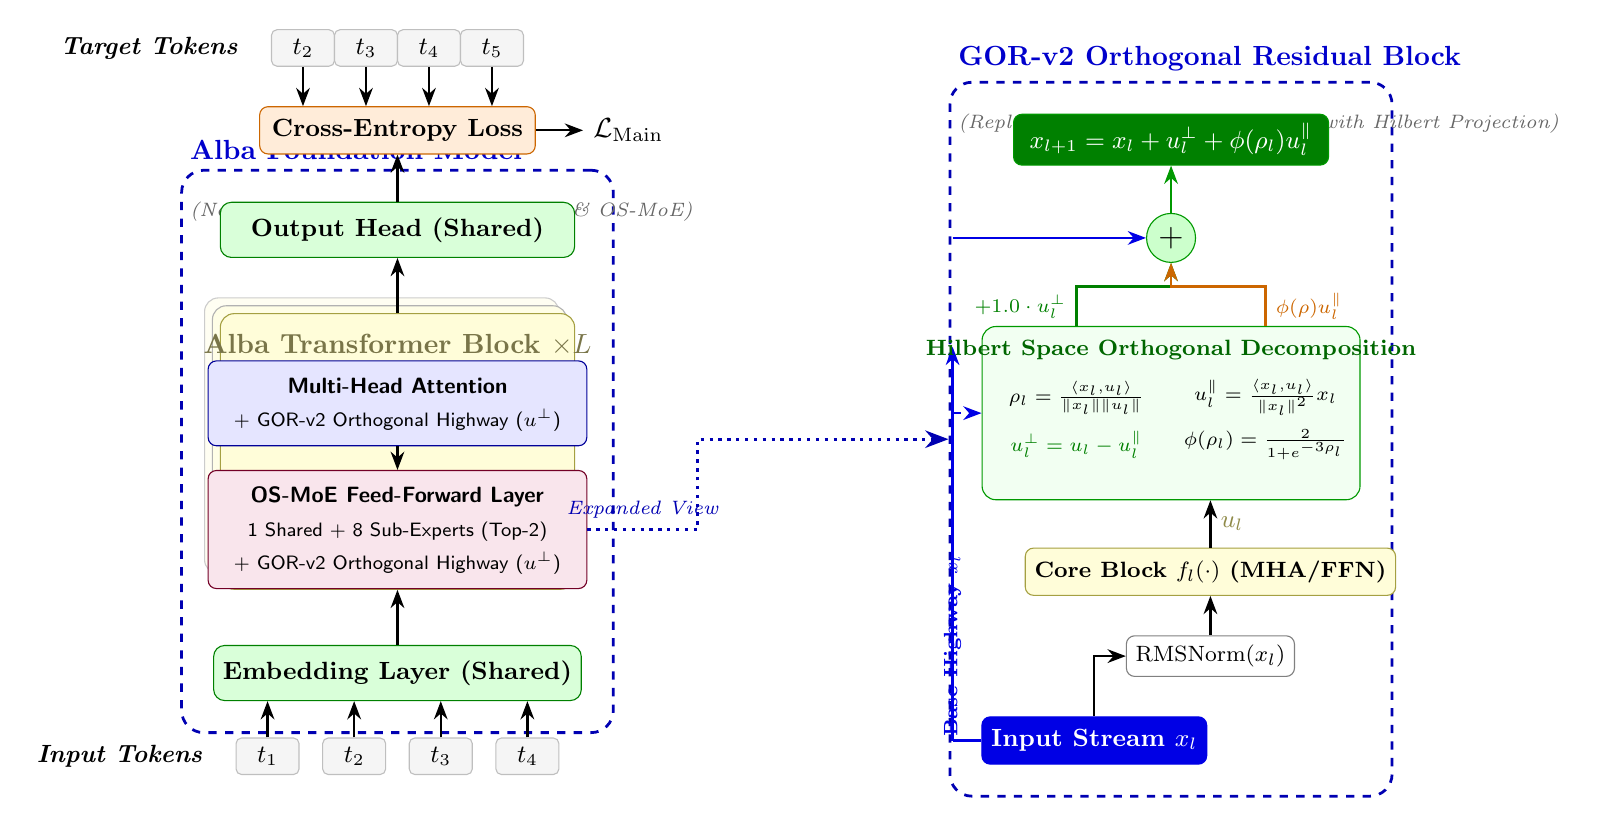
\begin{tikzpicture}[
    >=Stealth,
    font=\sffamily,
    token/.style={draw=black!25, fill=black!4, rounded corners=2pt, minimum width=0.8cm, minimum height=0.45cm, font=\small\itshape},
    head/.style={draw=green!50!black, fill=green!15, rounded corners=4pt, minimum width=4.5cm, minimum height=0.7cm, font=\bfseries\small},
    block/.style={draw=yellow!60!black, fill=yellow!15, rounded corners=5pt, minimum width=4.5cm, minimum height=3.5cm},
    norm/.style={draw=black!50, fill=white, rounded corners=3pt, minimum width=1.8cm, minimum height=0.5cm, font=\footnotesize},
    loss/.style={draw=orange!80!black, fill=orange!15, rounded corners=3pt, minimum width=3.5cm, minimum height=0.6cm, font=\bfseries\small},
    frame/.style={draw=blue!70!black, dashed, rounded corners=8pt, line width=1pt}
]

    % ==================== MAIN MODEL (LEFT) ====================
    % Input Tokens
    \node[token] (t1) at (0, 0) {$t_1$};
    \node[token] (t2) at (1.1, 0) {$t_2$};
    \node[token] (t3) at (2.2, 0) {$t_3$};
    \node[token] (t4) at (3.3, 0) {$t_4$};
    \node[left=0.3cm of t1, font=\bfseries\itshape\small] {Input Tokens};

    % Embedding
    \node[head, above=0.7cm of $(t2)!0.5!(t3)$] (emb) {Embedding Layer (Shared)};
    \draw[->, thick] (t1.north) -- (t1.north |- emb.south);
    \draw[->, thick] (t2.north) -- (t2.north |- emb.south);
    \draw[->, thick] (t3.north) -- (t3.north |- emb.south);
    \draw[->, thick] (t4.north) -- (t4.north |- emb.south);

    % Stacked Transformer Cards
    \node[block, fill=yellow!5, draw=black!20, above=0.7cm of emb, xshift=-0.2cm, yshift=0.2cm] (stack2) {};
    \node[block, fill=yellow!10, draw=black!30, above=0.7cm of emb, xshift=-0.1cm, yshift=0.1cm] (stack1) {};
    \node[block, above=0.7cm of emb] (mainblock) {};
    \draw[->, thick] (emb) -- (mainblock);

    \node[font=\bfseries, color=yellow!40!black] at ($(mainblock.north)+(0,-0.4)$) {Alba Transformer Block $\times L$};
    
    % Internal Sub-blocks
    \node[draw=blue!60!black, fill=blue!10, rounded corners=3pt, minimum width=3.8cm, minimum height=0.8cm, below=0.6cm of mainblock.north] (mha) {
        \begin{tabular}{c}
            \textbf{\footnotesize Multi-Head Attention} \\
            \scriptsize + GOR-v2 Orthogonal Highway ($u^\perp$)
        \end{tabular}
    };
    \node[draw=purple!60!black, fill=purple!10, rounded corners=3pt, minimum width=3.8cm, minimum height=1.1cm, below=0.3cm of mha] (moe) {
        \begin{tabular}{c}
            \textbf{\footnotesize OS-MoE Feed-Forward Layer} \\
            \scriptsize 1 Shared + 8 Sub-Experts (Top-2) \\
            \scriptsize + GOR-v2 Orthogonal Highway ($u^\perp$)
        \end{tabular}
    };
    \draw[->, thick] (mha) -- (moe);

    % Output Head
    \node[head, above=0.7cm of mainblock] (head) {Output Head (Shared)};
    \draw[->, thick] (mainblock) -- (head);

    % Loss
    \node[loss, above=0.6cm of head] (loss) {Cross-Entropy Loss};
    \draw[->, thick] (head) -- (loss);
    \draw[->, thick] (loss.east) -- ++(0.6, 0) node[right, font=\bfseries] {$\mathcal{L}_{\mathrm{Main}}$};

    % Target Tokens
    \node[token, above=0.5cm of loss, xshift=-1.2cm] (tg2) {$t_2$};
    \node[token, above=0.5cm of loss, xshift=-0.4cm] (tg3) {$t_3$};
    \node[token, above=0.5cm of loss, xshift=0.4cm] (tg4) {$t_4$};
    \node[token, above=0.5cm of loss, xshift=1.2cm] (tg5) {$t_5$};
    \draw[->, thick] (tg2) -- (tg2 |- loss.north);
    \draw[->, thick] (tg3) -- (tg3 |- loss.north);
    \draw[->, thick] (tg4) -- (tg4 |- loss.north);
    \draw[->, thick] (tg5) -- (tg5 |- loss.north);
    \node[left=0.3cm of tg2, font=\bfseries\itshape\small] {Target Tokens};

    % Dashed Outer Frame
    \begin{scope}[on background layer]
        \node[frame, fit=(emb)(mainblock)(head), inner sep=0.4cm] (boxmain) {};
        \node[above right, font=\bfseries, color=blue!80!black] at (boxmain.north west) {Alba Foundation Model};
        \node[below right, font=\scriptsize\itshape, color=black!60] at ($(boxmain.north west)+(0,-0.3)$) {(Next-Token Prediction with GOR-v2 \& OS-MoE)};
    \end{scope}

    % ==================== GOR-v2 DETAIL (RIGHT) ====================
    \begin{scope}[xshift=8.5cm]
        \node[draw=blue!90!black, fill=blue!90!black, text=white, rounded corners=3pt, minimum width=2.4cm, minimum height=0.6cm, font=\bfseries\small] (inx) at (2, 0.2) {Input Stream $x_l$};
        
        \coordinate (skipleft) at (0.2, 0.2);
        \draw[thick, color=blue!90!black] (inx.west) -- (skipleft);
        \draw[->, thick, color=blue!90!black] (skipleft) -- ++(0, 5.0) node[midway, left, font=\bfseries\scriptsize, rotate=90] {Base Highway $x_l$};

        \node[norm, above right=0.5cm and 0.4cm of inx.north] (rnorm) {RMSNorm($x_l$)};
        \draw[->, thick] (inx.north) |- (rnorm.west);

        \node[draw=yellow!60!black, fill=yellow!15, rounded corners=3pt, minimum width=3.0cm, minimum height=0.6cm, above=0.5cm of rnorm, font=\bfseries\footnotesize] (core) {Core Block $f_l(\cdot)$ (MHA/FFN)};
        \draw[->, thick] (rnorm) -- (core);

        % Hilbert Engine
        \node[draw=green!60!black, fill=green!5, rounded corners=5pt, minimum width=4.8cm, minimum height=2.2cm, above=0.6cm of core, xshift=-0.5cm] (hilbert) {};
        \draw[->, thick] (core.north) -- (core.north |- hilbert.south) node[midway, right, font=\bfseries\small, color=yellow!50!black] {$u_l$};
        
        \node[font=\bfseries\footnotesize, color=green!40!black] at ($(hilbert.north)+(0,-0.3)$) {Hilbert Space Orthogonal Decomposition};
        \node[font=\scriptsize] at ($(hilbert.center)+( -1.2, 0.2)$) {$\rho_l = \frac{\langle x_l, u_l \rangle}{\|x_l\| \|u_l\|}$};
        \node[font=\scriptsize] at ($(hilbert.center)+( 1.2, 0.2)$) {$u_l^\parallel = \frac{\langle x_l, u_l \rangle}{\|x_l\|^2} x_l$};
        \node[font=\scriptsize\bfseries, color=green!50!black] at ($(hilbert.center)+( -1.2, -0.4)$) {$u_l^\perp = u_l - u_l^\parallel$};
        \node[font=\scriptsize] at ($(hilbert.center)+( 1.2, -0.4)$) {$\phi(\rho_l) = \frac{2}{1 + e^{-3\rho_l}}$};

        \draw[->, dashed, thick, color=blue!90!black] (skipleft |- hilbert.west) -- (hilbert.west);

        % Outputs
        \node[draw=green!60!black, fill=green!20, circle, inner sep=2pt, font=\bfseries\large, above=0.8cm of hilbert] (add) {$+$};

        \draw[->, thick, color=blue!90!black] (skipleft |- add.west) -- (add.west);
        \draw[->, thick, color=green!50!black] ($(hilbert.north)+(-1.2, 0)$) -- ++(0, 0.5) node[midway, left, font=\scriptsize\bfseries] {$+1.0 \cdot u_l^\perp$} -| (add.south);
        \draw[->, thick, color=orange!80!black] ($(hilbert.north)+(1.2, 0)$) -- ++(0, 0.5) node[midway, right, font=\scriptsize\bfseries] {$\phi(\rho) u_l^\parallel$} -| (add.south);

        \node[draw=green!60!black, fill=green!50!black, text=white, rounded corners=3pt, minimum width=4.0cm, minimum height=0.6cm, font=\bfseries\small, above=0.6cm of add] (outx) {$x_{l+1} = x_l + u_l^\perp + \phi(\rho_l) u_l^\parallel$};
        \draw[->, thick, color=green!60!black] (add) -- (outx);

        \begin{scope}[on background layer]
            \node[frame, fit=(inx)(hilbert)(outx), inner sep=0.4cm] (boxdetail) {};
            \node[above right, font=\bfseries, color=blue!80!black] at (boxdetail.north west) {GOR-v2 Orthogonal Residual Block};
            \node[below right, font=\scriptsize\itshape, color=black!60] at ($(boxdetail.north west)+(0,-0.3)$) {(Replacing Classical Addition $x+u$ with Hilbert Projection)};
        \end{scope}
    \end{scope}

    \draw[->, dotted, line width=1.2pt, color=blue!70!black] (moe.east) -- ++(1.4, 0) node[midway, above, font=\scriptsize\itshape] {Expanded View} |- (boxdetail.west);

\end{tikzpicture}
\end{document}
